\documentclass[a4paper, 11pt, titlepage]{article}
\usepackage{ucs}
\usepackage[german,ngerman]{babel}
\usepackage{fontenc}
\usepackage[pdftex]{graphicx}
\usepackage{color}

\renewcommand*{\thesubsection}{\alph{subsection}.}

\begin{document}
\title{Datenbanken \\
Ausarbeitung \"Ubung 5}

\author{Jakob Schulz}

\date{6. November 2023}

\maketitle{\thispagestyle{plain}}

\section{Aufgabe}

\subsection{}
\begin{tabular}{lll}
Spalte&Datentyp&Zusatz\\
Taxa&varchar&not-null\\
Typ&varchar&not-null\\
Vouchers ID&varchar(1)\\
Botanical garden ID&varchar\\
Sample ID&varchar&\\
Origin&varchar&not-null\\
rpoB&varchar&\\
rpoC&varchar&\\
matK&varchar&\\
trnH-psbA&varchar&\\
rpl32-trnL&varchar&\\
\end{tabular}\\
\\
Die Spalte Typ hat nur wenige verschiedene Werte. ("`A"', "`H"', "`W"')\\
Die Spalte Vouchers ID lässt sich als Prim"arschl"ussel verwenden.
Es l"asst sich keinen Prim"arschl"ussel finden
\subsection{}
Formel: =MAX(LÄNGE("`Spalte ausw"ahlen"'))\\
\begin{tabular}{ll}
Spalte&Max. L"ange der Werte\\
Taxa&41\\
Typ&1\\
Vouchers ID&11\\
Botanical garden ID&21\\
Sample ID&9\\
Origin&68\\
rpoB&8\\
rpoC&8\\
matK&8\\
trnH-psb&8\\
rpl32-trnL&8\\
\end{tabular}\\
\subsection{}
Ursprüngliche Tabelle:
\begin{verbatim}
create table barcodes (
id int generated always as identity primary key,
taxon varchar(20) not null,
type varchar(1),
voucherID varchar(12),
gardenID varchar(12),
sampleID varchar(12),
origin varchar(50),
rpoB varchar(12),
rpoC varchar(12),
matK varchar(12),
trnHpsbA varchar(12),
rpl32 varchar(12)
\end{verbatim}
Korrigierte Tabelle:
\begin{verbatim}
create table barcodes (
id int generated always as identity primary key,
taxon varchar(41) not null,
type varchar(1),
voucherID varchar(11),
gardenID varchar(21),
sampleID varchar(9),
origin varchar(68),
rpoB varchar(8),
rpoC varchar(8),
matK varchar(8),
trnHpsbA varchar(8),
rpl32 varchar(8)
)
\end{verbatim}

\section{Aufgabe}
\subsection{}
\begin{verbatim}
insert into barcodes(taxon, type, voucherid, gardenid, sampleid, 
origin, rpob, rpoc, matk, trnhpsba, rpl32)(
Select*
from csvread('C:\Users\jakob\Desktop\Hochschule Furtwangen\1. Semester
\Datenbanken\Aufgaben\Aufgabe 5\barcodes.csv'))
\end{verbatim}
\subsection{}
Anweisung:
\begin{verbatim}
Select*
from barcodes
\end{verbatim}
Ergebnis:\\
\includegraphics [width = 13cm]{ImpotierteDatensaetze_Ausschnitt}\\
\subsection{}
Befehl:
\begin{verbatim}
Select Distinct Taxon
from barcodes
\end{verbatim}
Taxon ist hierbei eine Spalte. Um nun zu "uberpr"ufen, ob eine Spalte Doubletten besitzt, muss man jede Spalte der Tabelle in den obigen Aufruf einsetzen. Das RDBMS gibt zus"atzlich zu den gefundenen Daten auch die Anzahl der gefundenen Daten aus. Ist diese kleiner, als die Gesamtanzahl (255 Datens"atze insgesamt), so ent"alt die Spalte Doubletten.\\
\textcolor{red}{Wichtig: Mehrere "`Null"'- Werte sind keine Doubletten.
M"ochte man nur die Doubletten, dann muss man select count(distinct taxon). Hiermit wird "`null"' nicht beachtet!\\
(Ansonsten k"onnte es m"oglich sein, dass man denkt, dass taxon doubletten hat, obwohl lediglich alle anderen nicht ausgegebenen und gez"ahlten Werte null sind.)}\\
\\
Die Spalte Taxon enth"alt Doubletten\\
Die Spalte type enth"alt Doubletten\\
Die Spalte voucherid enth"alt Doubletten\\
Die Spalte gardenid enth"alt Doubletten\\
Die Spalte sampleid enth"alt Doubletten\\
Die Spalte origin enth"alt Doubletten\\
Die Spalte rpob enth"alt Doubletten\\
Die Spalte matk enth"alt Doubletten\\
Die Spalte trnhpsba enth"alt Doubletten\\
Die Spalte rpl32 enth"alt Doubletten

\section{Aufgabe}
\subsection{}
Aufruf:
\begin{verbatim}
Select Count(Distinct taxon) AS Anzahl_Verschiedener_Werte
From barcodes
\end{verbatim}
Count: Count(distinct taxon): Z"ahlt verschiedene Werte der Spalte Taxon\\
AS Anzahl\_Verschiedener\_Werte: Gibt der ausgabetabelle einen Namen.\\
\\
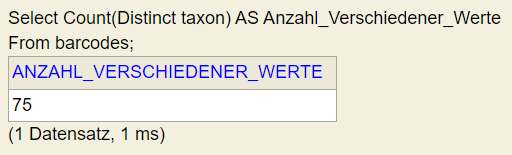
\includegraphics [width = 5cm]{Anzahl_verschiedener_Werte} 
\subsection{}
Korrigierte Tabelle:
\begin{verbatim}
create table taxa(
 id int generated always as identity primary key,
 name varchar(48) unique
)
\end{verbatim}
\subsection{}
Befehl:
\begin{verbatim}
insert into taxa(name)
Select Distinct taxon
from barcodes
\end{verbatim}
\subsection{}
Folgender Befehl gibt Anzahl der verschiedenen Namen in der Tabelle taxa:
\begin{verbatim}
Select Count(distinct name)
from taxa
\end{verbatim}
In der Tabelle Taxa sind 75 verschiedene Werte in der Spalte Namen abgespeichert. Dies entspricht der Anzahl der verschiedenen Werte der Spalte Taxon in der Tabelle Barcodes. (Siehe Aufgabe 3a Bild)\\
\\
Es kommen keine "uberfl"ussigen Werte mehr vor, denn folgende Befehle liefern die gleiche Anzahl an Datens"atzen:
\begin{verbatim}
Select Count(distinct name)
from taxa

Select Count(name)
from taxa
\end{verbatim}
Select Count(name) ber"ucksichtigt hierbei alle Datens"atze nicht nur die Doubletten.
\subsection{}
Befehl:
\begin{verbatim}
alter table barcodes add column taxonid int
\end{verbatim}
Die neue Spalte taxonid enth"alt keine Werte ("`null")\\
\subsection{}
Die ersten beiden Anweisungsbl"ocke erzeugen jeweils eine Tabelle mit einer Spalte des Types integer und einer Spalte des Types varchar.\\
Die update Anweisung f"ugt in die Spalte c11 (int)(Tabelle 1) alle Werte der Spalte c21 (Tabelle t2) ein, deren Werte c12(Tabelle t1) identisch mit den Werten c22(Tabelle t2) sind.
\subsection{}
Zuordnen der Werte:
\begin{verbatim}
update barcodes
set taxonid =(select id from taxa where name = taxon)
\end{verbatim}
\subsection{}
Fremdschl"ussel einf"ugen
\begin{verbatim}
alter table barcodes add foreign key(taxonid) references taxa(id)
\end{verbatim}
\subsection{}
Die Spalte taxon wird nicht mehr ben"otigt, da nun der Fremdschl"ussel taxon"id auf die Tabelle taxa verweist, welche die passenden Namen enth"alt.
\begin{verbatim}
alter table barcodes drop column taxon
\end{verbatim}
\end{document}